\documentclass[12pt,a4paper]{article}%
\usepackage[]{graphicx}\usepackage[]{color}
%% maxwidth is the original width if it is less than linewidth
%% otherwise use linewidth (to make sure the graphics do not exceed the margin)

%2multibyte Version: 5.50.0.2960 CodePage: 1252
\usepackage{amsfonts}
\usepackage{amssymb}
\usepackage[centertags]{amsmath}
\usepackage{graphicx}%
\usepackage{natbib}
\usepackage{color}
\usepackage[dvipsnames,svgnames*]{xcolor}
\usepackage{array}
\usepackage[hidelinks]{hyperref}
\usepackage[font=small,skip=5pt]{caption}
\usepackage[aboveskip=2pt]{subcaption}
\usepackage{amsmath}
\usepackage[]{algorithm2e}
\usepackage{amsthm}
\usepackage{url}
\usepackage{wasysym}
\usepackage{ulem}
\usepackage{afterpage}
\usepackage{bbm}
\setcounter{MaxMatrixCols}{30}
\providecommand{\U}[1]{\protect\rule{.1in}{.1in}}
\newtheorem{theorem}{Theorem}
\newtheorem{acknowledgement}[theorem]{Acknowledgement}
\newtheorem{axiom}[theorem]{Axiom}
\newtheorem{case}[theorem]{Case}
\newtheorem{claim}[theorem]{Claim}
\newtheorem{conclusion}[theorem]{Conclusion}
\newtheorem{condition}[theorem]{Condition}
\newtheorem{conjecture}[theorem]{Conjecture}
\newtheorem{corollary}[theorem]{Corollary}
\newtheorem{criterion}[theorem]{Criterion}
\newtheorem{definition}[theorem]{Definition}
\newtheorem{example}[theorem]{Example}
\newtheorem{exercise}[theorem]{Exercise}
\newtheorem{lemma}[theorem]{Lemma}
\newtheorem{notation}[theorem]{Notation}
\newtheorem{problem}[theorem]{Problem}
\newtheorem{proposition}[theorem]{Proposition}
\newtheorem{remark}[theorem]{Remark}
\newtheorem{solution}[theorem]{Solution}
\newtheorem{summary}[theorem]{Summary}
\setlength{\topmargin}{0in}
\setlength{\oddsidemargin}{0.1in}
\setlength{\evensidemargin}{0.1in}
\setlength{\textwidth}{6.5in}
\setlength{\textheight}{8.25in}
\numberwithin{equation}{section}
\title{Real Time Variational Density Forecasts}
\author{Nathaniel Tomasetti, Catherine Forbes and Anastasios Panagiotelis}
\begin{document}

\maketitle
\tableofcontents
\section{Introduction} 

Electricity prices have been subject to an extensive forecasting literature, as detailed in \citet{Weron2014}, and can be extremely volatile. For the 2012-2015 period in Victoria, the mean price was X/KWH but on X occaisions the price spiked upwards several orders of magnitude to upwards of $1,000/KWH, reaching as high as $10,000/KWH on X date. For this reason market participants are increasingly interested in a predictive density forecast, as the probability that the price will rise above a particular threshold in the next time period is more important than the mean value. To calculate a suitably accurate predictive density the Bayesian methodology is to be adopted in this thesis, as it can average over parameter and model uncertainty that is often ignored in frequentist methods. See \citet{Geweke2006} for a review on Bayesian forecasting and \citet{Gneiting2014} for density forecasting in general. 

Bayesian methods are computationally complex as they require integration over the set of unknown parameters, which must be large in a model that can capture the strong seasonal patterns in short term electricity load \citep{Taylor2003}, which is the main driver for electricity price and the focus of this work. To avoid this problem there are a range of techniques available to obtain the predictive distribution which do not involve integration, notably Markov Chain Monte Carlo (MCMC) methods. While MCMC has very strong convergence properties, computation is slow for even moderately complex models, which is problematic as Electricity demand in Victoria operates on a five minute interval. The predictive density for the next period's electricity load may not be available before it is observed.

Alternatives to MCMC include Variational Bayes (VB) and Expectation Propogation (EP), which aim to substitute the true posterior distribution for a vector of unknown parameters $\theta$, denoted by $p(\theta | y)$, with some approximate distribution denoted by $q(\theta | \lambda)$. Here $\lambda$ is a set of auxillary parameters associated with the approximation and not the model. For example, if $q(\theta | \lambda)$ is Gaussian $\lambda$ would be the mean and variance that parameterise $q$. Variational Bayes will be explored as an alternative computation strategy to MCMC in the context of short term electricity load forecasting using data from the 2012-2015 period in Victoria. The advantages in computation time for VB will be compared to the loss of statisitcal accuracy associated with the use of an approximation of the posterior instead of the truth. 

\section{Bayesian Inference}

Exact Bayesian inference in the context of forecasting uses the predictive density of $Y_{T+1}$ conditioned on the observed series, $y_{t}, t = 1, \dots T$, which is denoted by $y_{1:T}$. The first step requires the posterior distribution of the model parameters $\theta$, $p(\theta | y)$, where

\begin{equation}
\label{posterior}
 p(\theta | y_{1:T}) = \frac{p(y_{1:T}|\theta)p(\theta)}{\int_\theta p(y_{1:T}|\theta)p(\theta) d\theta}.
\end{equation}

Generally the solution to (\ref{posterior}) is unavailable. This section will offer two alternatives, MCMC and VB.
MCMC is used to create a sample from $p(\theta | y)$, and any function of interest from $p(\theta | y$ can be found with the relevant function applied to the sample, while VB replaces $p(\theta | y)$ with an approximation $q(\theta | \lambda)$, choosing some family $q$ and auxillary parameters $\lambda$ to minimise the Kullback-Leibler divergence from $q(\theta | \lambda)$ to $p(\theta | y)$.

\subsection{Markov Chain Monte Carlo}

There are many types of MCMC algorithm, the most common being a Gibbs sampler which iteratively samples from a $k$ dimensional parameter vector $\theta$ via the conditional distributions

\begin{align}
&p(\theta_1 | \theta_2, \dots, \theta_k, y_{1:T}) \nonumber \\
&p(\theta_2 | \theta_1, \theta_3, \dots, \theta_k, y_{1:T}) \nonumber \\
&\vdots \nonumber \\
&p(\theta_k | \theta_1, \dots, \theta_{k-1}, y_{1:T}). \nonumber
\end{align}

With enough iterations, these samples converge in distribution to $p(\theta | y)$ and can be used for inference. The computation time per iteration and number of iterations required for convergence is problem specific but typically increases with model complexity. 

To illustrate issues involved consider a simple auto-regressive time series model which will be used in the remainder of this section. This model is described by

\begin{equation}
\label{AR2}
y_t = \rho_1 y_{t-1} + \rho_2 y_{t-2} + \epsilon_t
\end{equation}

where $\epsilon_t \sim \mathcal{N}(0, \sigma^2)$. The likelihood of parameters $\theta = (\rho_1, \rho_2m \sigma^2)'$ is given by

\begin{align}
\label{likelihood}
L(\theta | y_{1:T}) &= p(y_1, y_2 | \theta) \prod_{t=3}^{T}p(y_t | y_{1:t-1}, \theta) \nonumber \\
&= \frac{1}{(2\pi)} |\Sigma|^{-1/2} \sigma^{-(T-2)} \exp \left\{ \frac{-1}{2} \left( \textbf{y}' \Sigma^{-1} \textbf{y} + \frac{1}{\sigma^2} \sum_{t=3}^{T}(y_t - \phi_1 y_{t-1} - \phi_2 y_{t-2})^2 \right) \right\}
\end{align}

where 

\begin{equation}
\Sigma = \left[ \begin{array}{cc} \gamma(0) & \gamma(1) \\ \gamma(1), \gamma(0) \end{array} \right],\
\end{equation}

$\gamma(k)$ is the $k-th$ autocorrelation and $\textbf{y} = (y_1, y_2)'$.

The priors 

\begin{align}
p(\sigma^2) &\propto \sigma^{-2} \nonumber \\
p(\rho_1, \rho_2) &\propto \mathbb{I}(\rho_2 > -1)\mathbb{I}(\rho_2 < 1 + \rho_1) \mathbb{I}(\rho_2 < 1 - \rho_1) \nonumber
\end{align}

are used, where $\mathbb{I}$ is the indicator and $p(\rho_1, \rho_2)$ defines the AR(2) stationary region.

The conditional distribution $p(\sigma^2 | y, \phi_1, \phi_2)$ is Inverse Gamma, while the conditionals for both $\phi$ parameters are intractable and sampled using a Metropolis-Hastings step with truncated normal random walk proposals. The truncation ensures that draws are only taken from the AR(2) stationary region.

Note: Will make the picture later
\begin{figure}
\label{MCMC}
%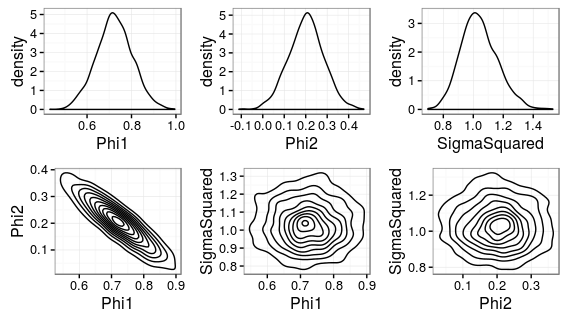
\includegraphics{MCMC.png}
\caption{MCMC draws for the AR(2) model with $T = 150, \phi_1 = 0.75, \phi_2 = 0.2$ and $\sigma^2 = 1$. Approximately 24\% of both $\phi$ parameters were accepted by the Metropolis Hastings step, then the first 50,000 draws were discarded and the remainder thinned to 1 in 300 to make dependence between draws negligible.}
\end{figure}

\subsection{Variational Bayes}

A faster alternative to MCMC is Variational Bayes, which introduces an approximating distribution $q(\theta | \lambda)$ choosing the functional form $q$ and given auxillary parameters $\lambda$ so that  misimises the Kullback-Leibler (KL) divergence \citep{Kullback1951} from $q(\theta | \lambda)$ the true posterior $p(\theta | y)$. The KL divergence is defined by

\begin{equation}
\label{KL-def}
KL[q(\theta | \lambda)||p(\theta | y)] = \int q(\theta | \lambda) \ln \left( \frac{q(\theta | \lambda)}{p(\theta | y)}\right) d\theta.
\end{equation}

The KL divergence is a non-negative, asymetric measure of the discrepancy between $p(\theta | y)$ and $q(\theta | \lambda)$ that will equal zero if and only if $p(\theta | y) = q(\theta | \lambda)$ almost everywhere \citep{Bishop2006}. Note that $KL[q(\theta | \lambda)||p(\theta | y)]$ can be expressed as

\begin{equation}
\label{KL-ELBO}
KL[q(\theta | \lambda)||p(\theta | y)] = \ln(p(y)) - \mathcal{L}(q, y)
\end{equation}

where $\mathcal{L}(q, y)$ is known as the Evidence Lower Bound (ELBO), defined by

\begin{equation}
\label{ELBO}
\mathcal{L}(q, y) = \int_{\theta} q(\theta|\lambda) \ln (p(y, \theta|\lambda)) d\theta -  \int_{\theta} q(\theta|\lambda) \ln (q(\theta|\lambda)) d\theta.
\end{equation}

Since $\ln(p(y))$ is constant given $y$, maximising (\ref{KL-ELBO}) with respect to $q$ is equivalent to minimising (\ref{KL-def}). Maximising the ELBO is much more convenient than minimising the KL Divergence, which can be seen in the following sections based on the two major implementations of Varitaional Bayes: Mean Field Variational Bayes and Stochastic Variational Bayes. Each of these take advantage of the functional form of the ELBO and offer computationally efficient algorithms to find a $q(\theta | \lambda)$ that is optimal within a particular clas of distributions. 

\subsubsection{Mean Field Variational Bayes} 



Mean Field Variational Bayes (MFVB) has origins in the physics literature \citep{Chandler1987} and restricts the search for an optimal approximating dististribution to the class of factorisable distributions

\begin{equation}
\label{mf1}
q(\theta|\lambda) = \prod_i^k q_i(\theta_i | \lambda_i).
\end{equation}

Each of the $k$ components $\theta_i$ may be a vector, but in most implementations are scalars. Each $\theta_i$ has an associated vector $\lambda_i$ which may be of a higher dimension than $\theta_i$. $\lambda_i$ is an auxillary parameter vector for the relevant factor $q_i$, which will be used in this section as shorthand notation for the distribution $q_i(\theta_i |\lambda_i)$. 

MFVB is widely used as it greatly simplifies maximisation of the ELBO (\citealp{Jordan1999}; \citealp{Bishop2006}), particularly in exponential family models \citep{Wainwright2008}.  Maximising the ELBO with respect to $q_i$ is as analytically involved as deriving the conditional distributions used in Gibbs based MCMC schemes, but the computation is simple. MFVB expresses (\ref{ELBO}) as a function of one $q_i$ only and then maximises with respect to that $q_i$. The final algorithm requires this to be repeated for each $i$ in $1, \dots, k$. Using the notation $q_{\setminus i} = \prod_{j\neq i}q_j$, \citet{Attias1999} shows that 

\begin{equation}
\label{mf2}
q(\theta_i | \lambda_i) \propto\exp( \mathbb{E}_{q_{\setminus i}} [\ln(p(y,\theta))])
\end{equation}

For illustration, consider data $y_i, i = 1, \dots, n$ generated from a $\mathcal{N}(\mu, \sigma^2)$ distribution where $p(\mu) \sim \mathcal{N}(\gamma, \lambda)$ and $p(\sigma^2) \sim Inv.Gamma(\alpha, \beta)$. It can be shown that

\begin{equation}
\label{mf3}
q(\mu) \propto \exp \left\{ \frac{-(n\lambda + \mathbb{E}(\sigma^{-2}))}{2\lambda\mathbb{E}(\sigma^{-2})} \left( \mu - \frac{\mathbb{E}(\sigma^{-2})\gamma + \lambda \sum_{i=1}^{n} y_i}{n \lambda + \mathbb{E}(\sigma^{-2})} \right) \right\}
\end{equation}

and

\begin{equation}
\label{mf4}
q(\sigma^2) \propto \sigma^{-2(n/2 + \alpha + 1)} \exp \left\{ \frac{ -1/2(\sum_{i=1}^{n}y_i^2 + \mathbb{E}(\mu^2) - 2 y_i \mathbb{E}(\mu)) - \beta}{\sigma^2} \right\}.
\end{equation}

It is evident that $q(\mu | \lambda) \sim \mathcal{N}(\tilde{\gamma}, \tilde{\lambda})$ and $q(\sigma^2 | \lambda) \sim Inv.Gamma(\tilde{\alpha}, \tilde{\beta})$. The parameters $\lambda = (\tilde{\gamma}, \tilde{\lambda}, \tilde{\alpha}, \tilde{\beta})'$ can be found by the set of mean field equations:

\begin{align}
\tilde{\gamma} &= \frac{\alpha / \beta \gamma + \lambda \sum_{i=1}^{n} y_i} {n \lambda + \alpha / \beta} \label{mf5} \\ 
\tilde{\lambda} &= \frac{n \alpha / \beta}{n \lambda + \alpha / \beta} \\
\tilde{\alpha} &= \frac{n}{2} + \alpha \\
\tilde{\beta} &= \frac{1}{2} \left(\sum_{i=1}^{n} y_i^2 + n(\tilde{\gamma}^2 + \tilde{\lambda}) - 2 \sum_{i=1}^{n} y_i \tilde{\gamma} \right) + \beta. \label{mf6}
\end{align}.

As there is a circular dependence in these equations an algorithm that cycles through each auxillary parameter until convergence to some pre-specified threshold is required.

In the event that (\ref{mf2}) is from an unrecognisable distribution a further approximation can be used, substituting in another distribution for the problematic $\tilde{q_i(\theta_i|\lambda_i)}.$ One method in \citet{Friston2006} uses a Laplace approximation to substitute a Gaussian distribution for these unrecognizable $q_i(\theta_i | \lambda_i)$, though the only requirement is that the substitute has an expectation that is a tractable function of its parameters to be used in (\ref{mf2}). 

Matching distributions in this way is a very similar method to finding the posterior conditional distribution, $p(\theta_i | y, \theta_{\setminus i}$ in a Gibbs MCMC scheme, with dependence on other parameters replaced by their expectations. The optimal approximating family for $\theta_i$, $q(\theta_i | \lambda_i)$, will come from the same distributional family as the conditional distribution $p(\theta_i | \theta_{j \neq i}, y)$, if it exists in a recognisable form such as the exponential family. The secondary level of approximations is analogous to the requirement of a Metropolis-Hastings-within-Gibbs step in MCMC to handle unrecognisable distributions.
\vspace{5mm}

The required algorithm is known as a coordinate ascent algorithm, and is described below where $\lambda$ is a $p$ dimensional vector.

\vspace{2mm}

\begin{algorithm}[H]
 \SetKwInOut{Input}{Input}
 \Input{Log Joint Density}
 \KwResult{Mean Field Approximation}
 Use (\ref{mf3}) to match each $q(\theta_i|\lambda_i)$ to a tractable distribution, or substitute a further approximation if neccesary.\;
 Derive the set of mean field equations such as in (\ref{mf5}) - (\ref{mf6}).\;
 Initialise $\lambda$ randomly. \;
 \While{Not converged}{
  \For{$i =  1$ \KwTo $k$}{
      Hold $\lambda_{j \neq i}$ fixed\;
      Update $\lambda_i$ using the relevant mean field equation.
     }
 }
 \caption{Coordinate Ascent for MFVB}
  \label{alg:algorithm1}
\end{algorithm}

\subsubsection{Stochastic Variational Bayes}

Restricting the approximating distribution to a factorisable family may be unsatisfactory in many applications where the dependence between parameters is important, as in the AR(2) model where Figure (\ref{MCMC}) shows strong dependence between $\phi_1$ and $\phi_2$. Without factorisation the simple method to maximise the ELBO as in MFVB is unavailable. \citet{Paisley2012} and \citet{Ranganath2014} have adapted a gradient ascent algorithm for use in Variational Bayes, resulting in what is known as Stochastic Variational Bayes (SVB).

The algorithm for SVB iteratively takes the  derivative of $\mathcal{L}(q(\theta | \lambda), y)$ in (\ref{ELBO}) with respect to $\lambda$ and the following updating step is applied until the ELBO converges to a maximum.

\begin{equation}
\label{SGA1}
\lambda^{(m+1)} = \lambda^{(m)} + \rho^{(m)} \nabla_{\lambda} \mathcal{L}(q(\theta | \lambda^{(m)}), y),
\end{equation}

where $\nabla_{\lambda}\mathcal{L}(q(\theta | \lambda^{(m)}), y)$ is the vector of partial derivatives of $\mathcal{L}(q(\theta | \lambda^{(m)}), y)$ with respect to each element of $\lambda$. This update requires some initial values $\lambda^{(0)}$ and a sequence $\rho^{(m)}, m = 1, 2, \dots$ known as the learning rate. If $\rho^{(m)}$ is chosen to satisfy the following conditions the algorithm is guaranteed to converge to a local maximum \citep{Robbins1951}.

\begin{align}
\sum_{m=1}^{\infty} \rho^{(m)} &=  \infty \\
\sum_{m=1}^{\infty} (\rho^{(m)})^2 &<  \infty.
\end{align}

Whilst a global maximum is desired, the ELBO is a high dimensional problem specific function that makes finding the global maximum extremely difficult and often only a local maximum can be found. One option to alleiviate this problem is to start the algorithm at a range of initial values choose the converged value with the highest maximised ELBO and hence lowest KL divergence to the true posterior 

SVB can find only the optimal values for $\lambda$ that are optimal for a distributional family $q$ that is specified by the user. To run SVB many choices of $q$ may be used and one selected on the basis of the highest ELBO. $q(\theta | \lambda)$ is restricted to the family of distributions that satisfy the condition that the order of differentation of the ELBO with respect to $\lambda$ and integration with respect to $\theta$ are interchangable, and SVB can only be applied to models where the log likelihood for $y$ is able to be evaluated. Given these conditions \citet{Ranganath2014} showed that a Monte Carlo estimate of the derivative of the ELBO can be taken by

\begin{equation}
\label{SGA2}
\nabla_{\lambda}\mathcal{L}(q(\theta | \lambda^{(m)}) \approx \frac{1}{S}\sum_{s=1}^{S} \nabla_{\lambda} [\ln(q(\theta_s | \lambda^{(m)}))] (\ln (p(y, \theta_s)) - \ln(q(\theta_s | \lambda^{(m)})))
\end{equation}

where $s = 1, \dots, S$ indicates simulations from $q(\theta | \lambda^{(m)})$.

\citet{Duchi2011} introduced the AdaGrad algorithm which can be implemented within SVB to control $\rho^{(m)}$. AdaGrad allows each $\lambda_i$ to have an independent $\rho^{(m)}_i$ that is inversely proportional to the gradient, so $\lambda$ takes bigger steps in flat regions and smaller steps in steep regions. 

Let 

\begin{equation}
\label{SGA3}
G_i^{(m)} = \sum_{j = 1}^{m} \left(\nabla_{\lambda_i}\mathcal{L}(q(\theta | \lambda^{(m)})\right)^2,
\end{equation}

then each component's learning rate is defined as

\begin{equation}
\label{SGA4}
\rho^{(m)}_i = \eta \left(G_i^{(m)}\right)^{-1/2}
\end{equation}

for some tuning parameter $\eta$.

The resulting Stochastic Gradient Ascent algorithm proceeds below with a $p$ dimensional $\lambda$ vector.

\begin{algorithm}[H]
 \SetKwInOut{Input}{Input}
 \Input{Log Joint Density, Approximation family q}
 \KwResult{Variational Approximation}
 Initialise $\lambda$\;
 \While{Not converged}{
  Simulate $\theta^s$ for $s = 1, \dots S$ from $q(\theta|\lambda^{(m)})$\;
  \For{$i =  1$ \KwTo $p$}{
      Calculate $\nabla_{\lambda_i}$ from (\ref{SGA2})\;
      Update $G_i^{(m)}$ and $\rho^{(m)}_i$ from (\ref{SGA3}) and (\ref{SGA4})\;
      }
  Update $\lambda^{(m+1)}$ from (\ref{SGA1})\;
  Set $m = m + 1$\;
 }
 \caption{Stochastic Gradient Ascent for SVB}
  \label{alg:algorithm2}
\end{algorithm}


\subsection{Vine Copulas}

Armed with an algorithm to find the Variational Bayes optimal paramerters $\lambda$ for a distribution $q$, there is a requirement to have a distribution $q$ that is itself optimal. Copulas are a flexible tool for constructing these distributions, as they allow the dependence structure between parameters to be fit independently from the marginal distributions. \citet{Sklar1959} proves that any joint probability distribution can be written as the product of the marginals and a copula function,

\begin{equation}
\label{vc1}
p(\theta_1, \dots, \theta_k) = p(\theta_1) \dots p(\theta_k) c(P(\theta_1), \dots, P(\theta_k))
\end{equation}

where $p(\theta)$ is a pdf, $P(\theta)$ is a cdf, and $c(\cdot)$ is a copula. 

\citet{Joe1994} introduces the vine copula, a technique to factorise a high-dimensional copula into a set of bivariate copulas in a similar way to the factorisation of a joint distribution into a marginal and conditional distribution, for example

\begin{equation}
\label{vc2}
c(P(\theta_1), P(\theta_2), P(\theta_3)) = c(P(\theta_1), P(\theta_2)) \cdot c(P(\theta_1), P(\theta_3)) \cdot c(P(\theta_2), P(\theta_3) | P(\theta_1)).
\end{equation}

A copula for a $k$ dimensional $\theta$ can be replaced with $k(k-1)/2$ bivariate copulas arranged in a vine copula, greatly increasing the amount of flexibility available to fit a distribution. However there are $O(k!)$ ways to factorise the full copula and choose a family for each bivariate copula, so without detailed problem specific information the application of a vine copula to Stochastic Variational Bayes is difficult. \citet{Tran2015} implements Variational Bayes with a vine copula in what they call Copula Variational Bayes, but the dimension of $\theta$ was small in that case allowing an exhaustive search for the vine copula that maximised the ELBO. 

Given a sample of $\theta$, \citet{Diimann2013} provide an algorithm to select the best vine factorisation by maximising Kendell's Tau, and the best family for each bivariate copula by maximising an information criterion such as AIC. In the real-time forecasting models used for electricity load demand, MCMC samples of the posterior distribution are available, though often immediately out of date. The approach used in this thesis is to run an MCMC algorithm, thin the resulting draws until they are effectively independent, choose an optimal family for each marginal distribution by AIC, then run (Vine copula algorithm here) to infer an optimal vine copula. This results in an approximating distribution $q(\theta | \lambda)$ that can then be used in an SVB algorithm to update $q(\theta | \lambda)$ as more observations become available. MCMC can be ran simultaenously and the resulting sample can be used to check if the distribution $q$ should be changed. 

\subsection{Applying Stochastic Variational Bayes}

Using the approach described in section 2.3, an application of VC algorirhtm to the MCMC draws obtained in section 2.1 found the following distribution to be optimal by AIC.

\begin{itemize}
\item $q(\phi_1)$ - Gaussian marginal
\item $q(\phi_2)$ - Gaussian marginal
\item $q(\sigma^2)$ - Inverse Gamma marginal
\item $c(Q(\phi_1), Q(\phi_2))$ - Gaussian copula
\item $c(Q(\phi_1), Q(\sigma^2))$ - Independent
\item $c(Q(\phi_2), Q(\sigma^2) | Q(\phi_1))$ - Independent
\end{itemize}

Figure (\ref{VBfit}) shows that Stochastic Variational Bayes (blue) fit the MCMC (red) sample very closely.

\begin{figure}[h]
\label{VBfit}
\centering
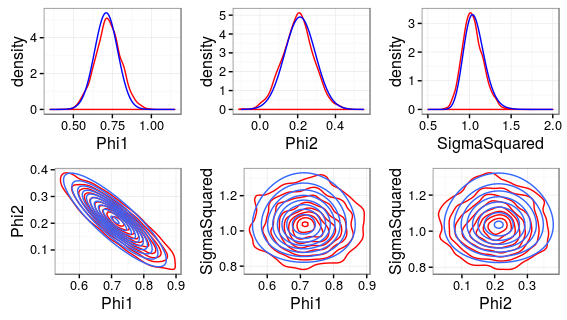
\includegraphics[scale = 0.5]{VBfit.png}
\caption{The fit of an SVB algorithm (red) compared to MCMC (red) for the AR(2) model described in section 2.1. SVB resulted in an almost identical posterior to MCMC while taking X less time to run. (working from home, will check runtime at uni)}
\end{figure}

\section{Electricity Load Forecasts}
\subsection{Motivation}

Note: Don't have data on hand, will do this section shortly

\begin{itemize}
\item Describe and plot load Data
\item Plot price data to emphasize price spikes
\item Follow up the intro to talk a bit about load forecasting
\end{itemize}

\subsection{Exponential Smoothing}

\citet{Taylor2003} explores the seasonal properties of electricity demand and introduces a double seasonal Holt-Winters exponential smoothing model with daily and weekly effects described by (\ref{ds-hw1})-(\ref{ds-hw4}), and later in \citet{Taylor2008} verifies that this approach is superior to other common time-series models for very short-term load forecasting \citep{Taylor2008}.

\begin{align}
y_t &= l_{t-1} + d_{t-m_1} + w_{t-m_2} + e_t \label{ds-hw1} \\
l_t &= \alpha (y_t - d_{t-m_1} - w_{t-m_2}) + (1 - \alpha)l_{t-1} \label{ds-hw2}\\
d_t &= \delta (y_t - l_{t-1} - w_{t-m_2}) + (1 - \delta)d_{t-m_1} \label{ds-hw3} \\
w_t &= \omega (y_t - l_{t-1} - d_{t-m_1}) + (1 - \omega)w_{t-m_2} \label{ds-hw4}
\end{align}

where $m_1$ and $m_2$ are the lengths of the daily and weekly cycle, restricting the smoothing parameters $\alpha, \delta, \omega$ to lie in $(0, 1)$. This can be rewritten as a single source of error state-space model \citep{Snyder1985},

\begin{align}
y_t &= l_{t-1} + d_{t-m_1} + w_{t-m_2} + e_t \label{ds-hw-ssoe1} \\
l_t &= l_{t-1} + \alpha e_t \label{ds-hw-ssoe2} \\
d_t &= d_{t-m_1} + \delta e_t \label{ds-hw-ssoe3} \\
w_t &= w_{t-m_2} + \omega e_t \label{ds-hw-ssoe4}. 
\end{align}

The unknown parameters are $\theta = (\alpha, \delta, \omega)', \sigma^2$ and $b_0 = (l_0, d_0, \dots, d_{-(m_1 - 1)}, w_0, \dots, w_{-(m_2 - 1)})'$ a $m_1 + m_2 + 1$ length vector of the initial states of the latent variables. 
\citet{Forbes2000} derives the marginal distribution $p(\theta | y)$ and notes that, conditioned on a draw of these parameters, the remaining unknown parameters can be sampled as a Bayesian linear regression problem. This method involves inverting a matrix that is singular using the parameterisation described by (\ref{ds-hw-ssoe1}) - (\ref{ds-hw-ssoe4}), but restricting the latent parameters via

\begin{align}
d_t &= - \sum_{i=1}^{m_1-1} d_{t-i} \\
w_t &= - \sum_{i=1}^{m_2-1} w_{t-i}
\end{align}

avoids this problem. The resulting model is described by

\begin{align}
y_t &= l_{t-1} - \sum_{i = 1}^{m_1 - 1}d_{t-i} - \sum_{i = 1}^{m_2 - 1}w_{t-i} + e_t \label{ds-hw-rp1} \\
l_t &= l_{t-1} + \alpha e_t \label{ds-hw-rp2} \\
d_t &= - \sum_{i = 1}^{m_1 - 1}d_{t-i} + \delta e_t \label{ds-hw-rp3} \\
w_t &= - \sum_{i = 1}^{m_2 - 1}w_{t-i} + \omega e_t \label{ds-hw-rp4}.
\end{align}

\citet{Forbes2000} recommends numerical integration of the marginal posterior density of $\theta$,

\begin{equation}
\label{exp-sm-marginal}
p(\theta | y_{1:T}) \propto \left| \widetilde{X}' \widetilde{X} \right|^{-1/2} \tilde{s}^{-(T-(m_1 + m_2 - 1))} p(\theta),
\end{equation}

where $\widetilde{X}$ and $\tilde{s}$ are functions of $\theta$ and $y$. The problems with using this method in our model are two-fold: repeating a three dimensional numerical integrion each time a new data point is observed within the five minute window is not feasible difficult, and the $T$ in the exponent makes most evalutions of $p(\theta | y_{1:T})$ computationally zero when $T$ is large. 

\begin{itemize}
\item Should try and get an exponential smoothing MCMC working using Metropolis-Hastings for $\theta$. Log densities help with the $T$ being too large problem but the grid is too large for numerical integration to be a good idea.
\end{itemize}

\section{Timeline}
\begin{itemize}
\item Put something here eventually
\end{itemize}

\bibliographystyle{asa}
\bibliography{references}

\end{document}
\grid
